\section{Spannungsreferenzen} 

\subsection{Verschiedene Arten der Rerferenzspannungserzeugung} 
	\begin{longtable}{|l|l|l|}
	\hline
		\begin{minipage}{4cm}
			\textbf{Einfachste "`Referenzspannungsquelle"'}
		\end{minipage}
	&
		\begin{minipage}{6cm}
			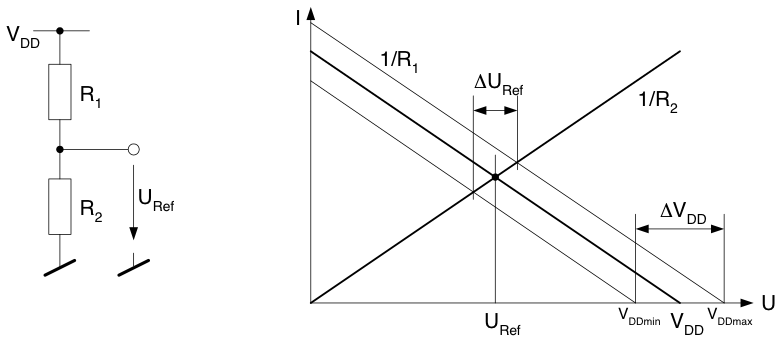
\includegraphics[width=6cm,trim=0 0 0 -5]{pictures/spannungsteiler}
		\end{minipage}
	&
		\begin{minipage}{8cm}
			\begin{equation*}
				S_{V_{DD}}^{U_{Ref}}=\frac{\frac{\Delta
				U_{Ref}}{U_{Ref}}}{\frac{\Delta V_{DD}}{V_{DD}}}=1
			\end{equation*}
			S: Sensitivität: Relative Änderung des Ausgangs zu Relativer Änderung des Eingangs
		\end{minipage}
	\\ \hline
		\begin{minipage}{4cm}
			\textbf{Dioden Referenz}
		\end{minipage}
	&
		\begin{minipage}{6cm}
			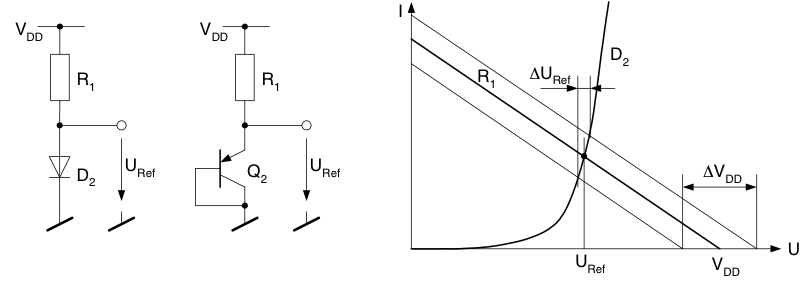
\includegraphics[width=6cm]{pictures/diodenReferenz}
		\end{minipage}
	&
		\begin{minipage}{8cm}
			\begin{gather*}
				U_{Ref}=U_{EB}=\frac{kT}{e}\ln{\frac{I}{I_{s}}} \notag\\
				\text{ für }V_{DD} \gg U_{EB}\\
				S_{V_{DD}}^{U_{Ref}}=\frac{1}{\ln{\frac{I}{I_{S}}}}<1
			\end{gather*}
		\end{minipage}
	\\ \hline
		\begin{minipage}{4cm}
			\textbf{MOSFET Referenz}
		\end{minipage}
	&
		\begin{minipage}{6cm}
			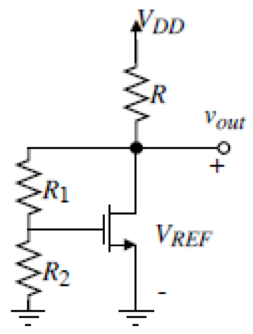
\includegraphics[width=2.5cm,trim=0 0 0 -5]{pictures/mosfetReferenz}
		\end{minipage}
	&
		\begin{minipage}{8cm}
			\begin{equation*}
				V_{REF}\approx \frac{R_{1}+R_{2}}{R_{2}}V_{GS}
			\end{equation*}
			\begin{equation*}
				V_{GS} \approx \text{ konst.}\quad\Leftrightarrow\quad V_{out} \text{ konst.}
			\end{equation*}
			$V_{GS}$ hat grosse Toleranzen $\Leftrightarrow$ eher unüblich
		\end{minipage}
	\\ \hline
		\begin{minipage}{4cm}
			\textbf{Bootstrap Referenz}
		\end{minipage}
	&
		\begin{minipage}{6cm}
			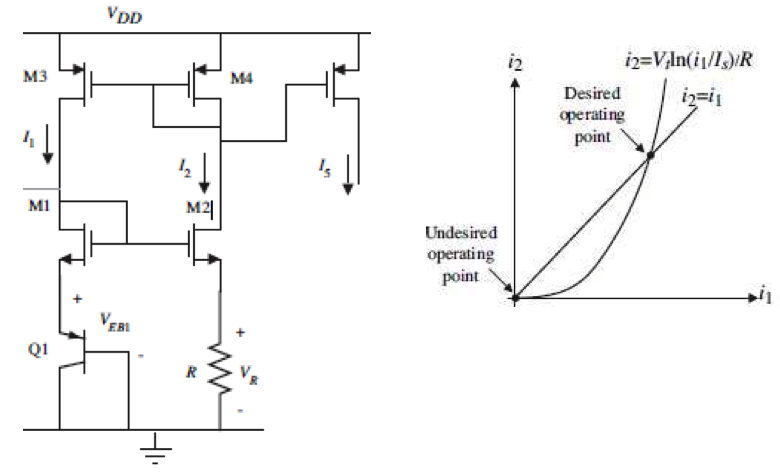
\includegraphics[width=6cm]{pictures/bootstrapReferenz}
		\end{minipage}
	&
		\begin{minipage}{8cm}
			\begin{gather*}
				I_{1}=I_{2} \\
				I_2 \cdot R = m \cdot  U_T \cdot \ln\left(\frac{I_1}{I_S}\right) \\
				U_{T}=\frac{kT}{q}
			\end{gather*}
				Stromspiegel (PTAT-Stromquelle) \\
				(PTAT: Proportional To Absolute Temperature)
			\end{minipage}
	\\ \hline
		\begin{minipage}{4cm}
			\textbf{Zenerdiode Referenz}
		\end{minipage}
		&
		\begin{minipage}{6cm}
			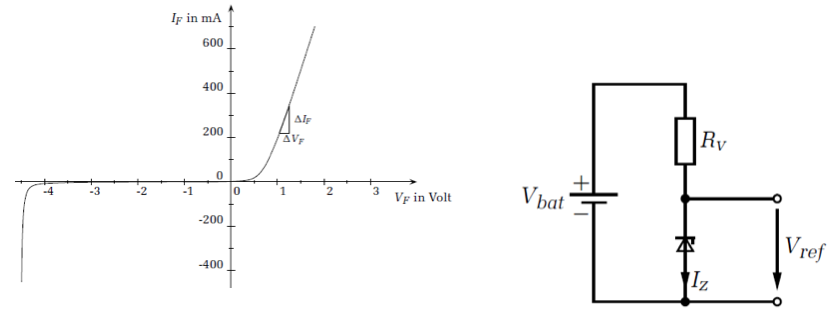
\includegraphics[width=6cm,trim=0 0 0 -5]{pictures/zenerReferenz}
		\end{minipage}
		&
		\begin{minipage}{8cm}
			Häufigste Spannung: $5,6V$ (minimaler Temperaturkoeffizient)
		\end{minipage}
	\\ \hline
		\begin{minipage}{4cm}
			\textbf{Bandgap Referenz}
		\end{minipage}
	&
		\begin{minipage}{6cm}
			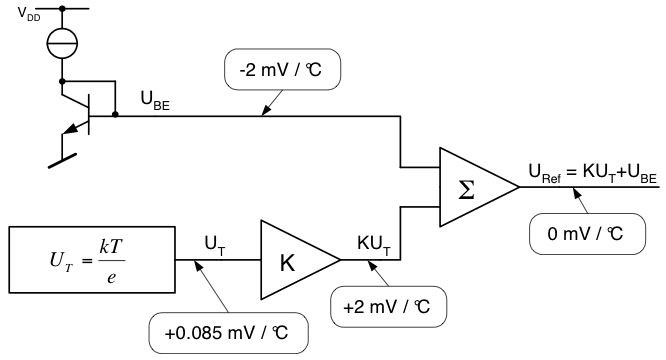
\includegraphics[width=6cm,trim=0 0 0 -5]{pictures/bandgapReferenz1}\\
			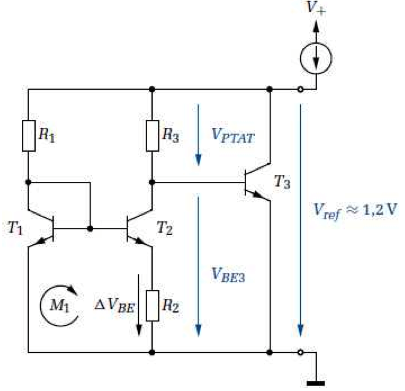
\includegraphics[width=6cm]{pictures/bandgapReferenz2}
		\end{minipage}
	&
		\begin{minipage}{8cm}
			Addition aus zwei Spannungen mit umgekehrten, 
			gleich grossen Temperatur-Koeffizienten:
			\begin{enumerate}
				\item Diodenspannung mit $-2 \frac{mV}{K}$ (hier: $U_{BE3}$)
				\item PTAT-Quelle mit $V_T=\frac{kT}{q} \Rightarrow +0.085 \frac{mV}{K}$
			\end{enumerate}

			\textbf{Herleitung:} \\
			Generell ist $I_C = B \cdot I_{BS} \left(e^{\frac{U_{BE}}{U_T}} -1 \right)
							\approx B \cdot I_{BS} \cdot e^{\frac{U_{BE}}{U_T}}$ \\
			Damit wird $\frac{I_{C1}}{I_{C2}}$ zu $e^{\frac{U_{BE1}-U_{BE2}}{U_T}}$ \\
			und $\Delta U_{BE} = U_{BE1}-U_{BE2} = U_T \ln\left(\frac{I_{C1}}{I_{C2}}\right)$ \\
			\\
			Ist das Verhältnis \smash{$\frac{I_{C1}}{I_{C2}}$} konstant, was beim Stromspiegel
			erfüllt ist, so hängt $\Delta U_{BE}$ wegen \smash{$U_T=\frac{k \cdot T}{q}$} nur 
			von der absoluten Temperatur $T$ ab ist somit eine PTAT-Quelle. \\
			\\
			Weil $I_{R3} \approx I_{R2}$ hängt auch $U_{PTAT}=I_{R3} \cdot R_3$ nur von der
			absoluten Temperatur $T$ und ist somit eine PTAT-Quelle. \\
			\\
			$U_{Ref} = U_{PTAT} + U_{BE3}$ ist also die Addition einer PTAT-Quelle und einer
			Diodenspannung und somit praktisch temperaturunabhängig mit 
			$U_{Ref} \stackrel{!}{\approx} 1,2V$. \\
			\\
			\textit{Oft als integrierte Bauteile erhältlich.}
		\end{minipage}
	\\ \hline
\end{longtable}

